\paragraph{La classe Starter}

\begin{minipage}
    {\linewidth}
    \centering
    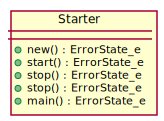
\includegraphics[width=0.30\linewidth]{../schemas/Conception_detaillee/classe_starter.pdf}
    \captionof{figure}{Diagramme de classe de Starter}
\end{minipage}

\subparagraph{Philosophie de conception \newline} 

\medspace

La classe Starter a pour rôle de créer et d'initialiser les classes qui seront utilisées par le programme {\nomLogiciel}.

Les objets créés sont les suivants :
\begin{itemize}
    \item UI,
    \item Sender
    \item Sniffer
    \item DriverCAN
    \item Postman
    \item Dispatcher
\end{itemize}

\subparagraph{Description structurelle \newline}

\medspace

\textbf{Attributs :}

N.A.

\textbf{Services offerts :}

\begin{itemize}
    \item \textbf{new() : ErrorState\_e} --- Opération qui crée les objets \textit{ui}, \textit{sender}, \textit{sniffer}, \textit{driverCAN}, \textit{dispatcher} et \textit{postman}.
    \item \textbf{start() : ErrorState\_e} --- Opération qui lance le programme {\nomLogiciel}.
    \item \textbf{stop() : ErrorState\_e} --- Opération qui arrête le programme {\nomLogiciel}.
    \item \textbf{free() : ErrorState\_e} --- Opération qui libère la mémoire allouée à l'objet Starter et à tous les objets qu'il a créés.
    \item \textbf{main() : int} --- Point d'entrée du programme. Opération qui instancie tous les objets et lance le programme {\nomLogiciel}.
\end{itemize}


\newpage 

\subparagraph{Séquence de démarrage et arrêt de {\nomLogiciel} \newline}

\medspace

\begin{minipage}
    {\linewidth}
    \centering
    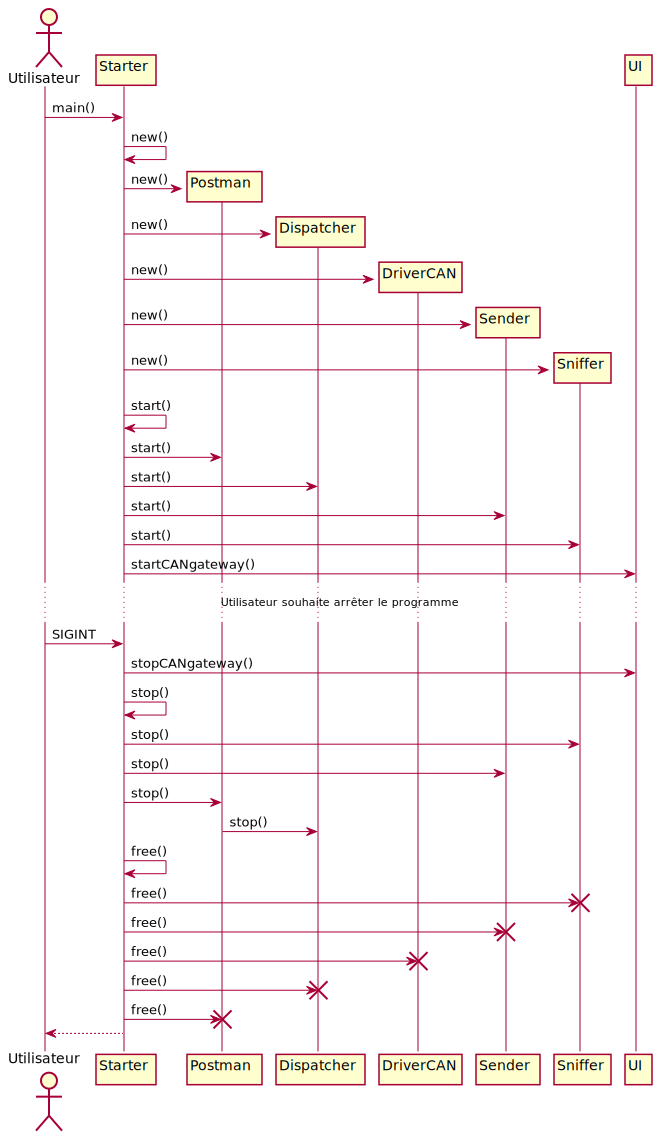
\includegraphics[height=0.9\textheight]{../schemas/Conception_detaillee/diag_sequence_Starter.pdf}
    \captionof{figure}{Diagramme de séquence de démarrage de {\nomLogiciel}}
\end{minipage}
